\chapter[Additional implementation]{Additional implementation details}
\chlab{implementation_extra}

Whereas the earlier implementation chapter~(\chref{implementation}) discussed \oframp{} at a higher, not too technical level, this chapter will discuss its technical details. Many descriptions rely on understanding of the network diagram that was presented in that chapter, in \figref{network_diagram} on \figpageref{network_diagram}.



\section[\oframp]{The Online tool for Fragment-based Molecule Parameterisation}
As can be seen in \figref{oframp_class}, a \verb|JavaScript| \verb|OFraMP| instance forms the heart of \oframp. This instance contains a \verb|settings| object containing the complete configuration for the system, a \verb|Behavior| implementation, and a \verb|MoleculeViewer|. These types, and all others in the class diagram, will be discussed in the next sections.

\begin{figure}
\center
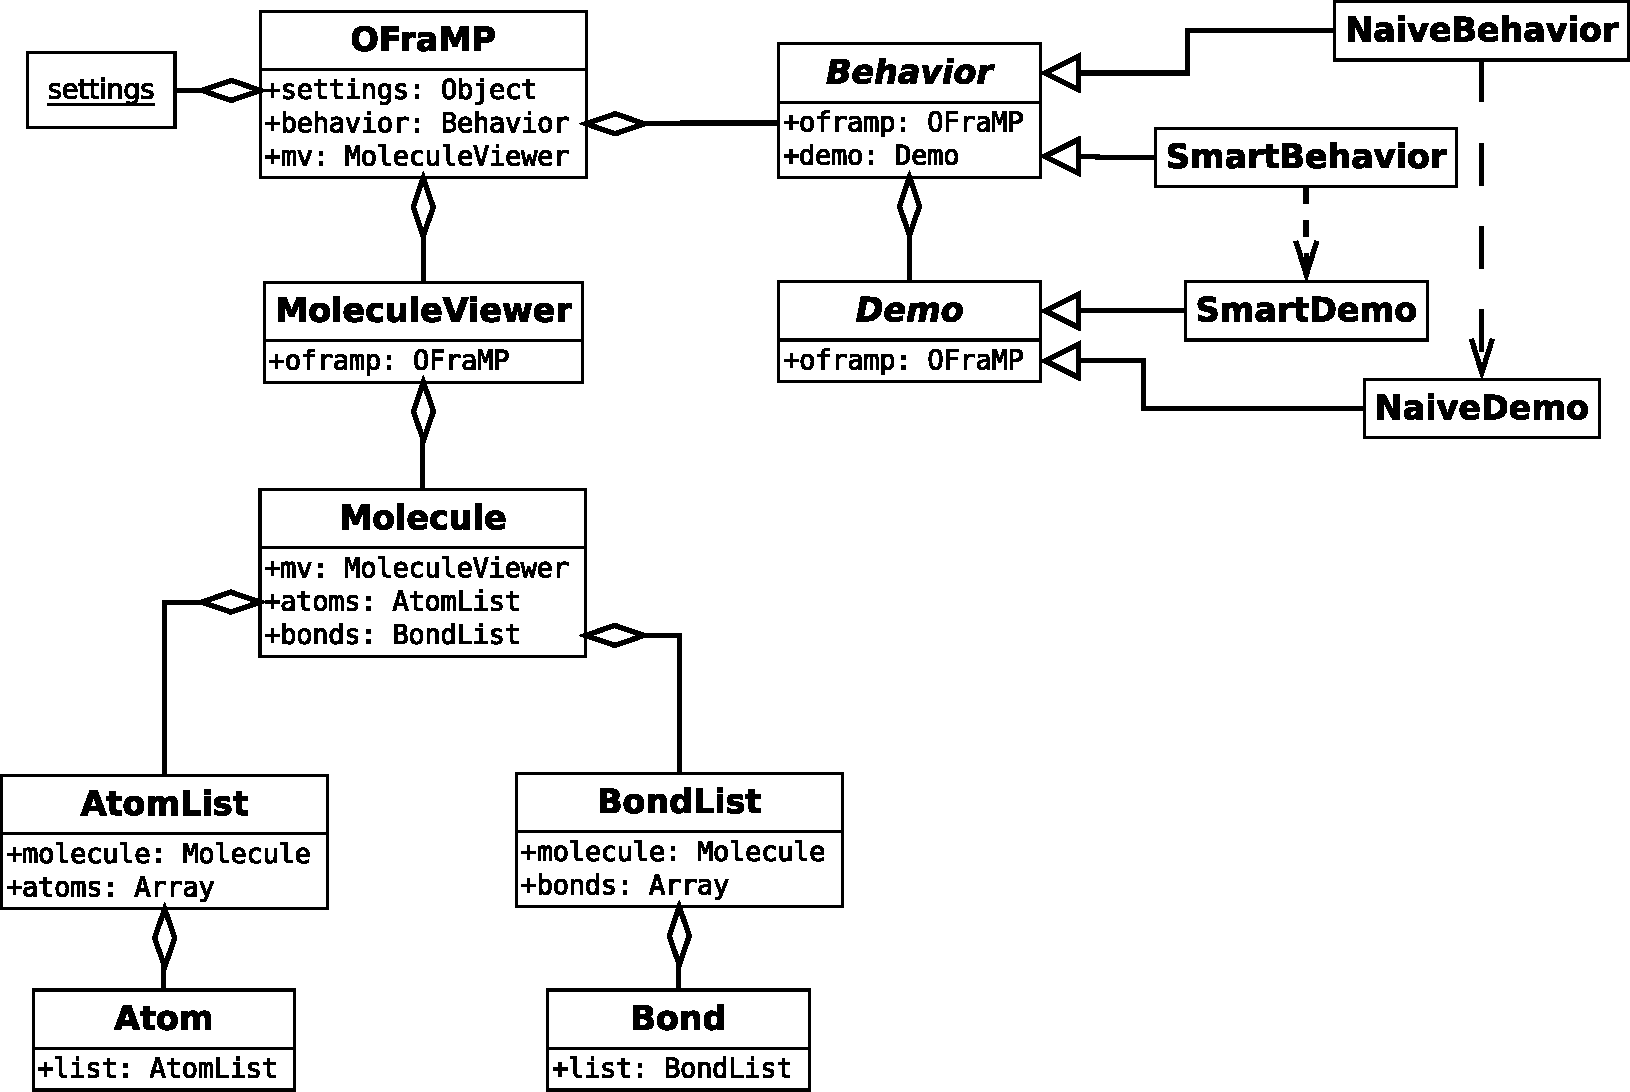
\includegraphics[width=\textwidth]{img/oframp_class.pdf}
\caption{Simplified class diagram of \oframp.}
\figlab{oframp_class}
\end{figure}


\subsection{Visualisation}
Once a molecule data string has been entered into the system, the positions of its atoms and the connections between them are retrieved from \oapoc~(see \secref{impl2_oapoc}). This data is then transformed to a \verb|JavaScript| \verb|Molecule| instance, as can be seen in \figref{oframp_class}. \verb|Molecule| instances can be visualised using a \verb|MoleculeViewer|, which will draw the molecule onto an \verb|HTML| \verb|canvas|.


\subsubsection{Deoverlapping}
As discussed in \secref{rw2_visualisation} and~\cite{clark2006structure}, overlap in atoms and bonds still occurs in modern molecule visualisation software. In the case of \oframp, where the atoms have a relatively large radius to make room for displaying the charge, chances are even higher. To temper the effects of this, a simple deoverlap algorithm has been implemented. \Figref{impl_deoverlap} shows the three different types of deoverlapping that \oframp{} can do. Here, the light blue line indicates a vector that is used to determine if there is any overlap, the red line indicates the overlapping part, and the green arrow~(of equal length to the red line) shows where the atom centre should be moved to in order to resolve the overlap.

By default, for performance reasons, only the deoverlapping of atoms is enabled. This is the easiest to detect and solve, but also the most important one. Atoms that overlap almost entirely might not be spotted by the user, and atom types and charges may become hidden due to another atom lying on top of them. As can be seen in \figref{impl_deoverlap}, this type of deoverlap works by calculating the distance between the two atom centres and subtracting the atom radius from that twice~(once for each atom). If this distance is smaller than $0$, both atom centres will be moved along the line that connects the two for a distance that is equal to the overlap distance. This ensures that the atoms will no longer overlap, and even creates some room between them.

\begin{figure}
\center
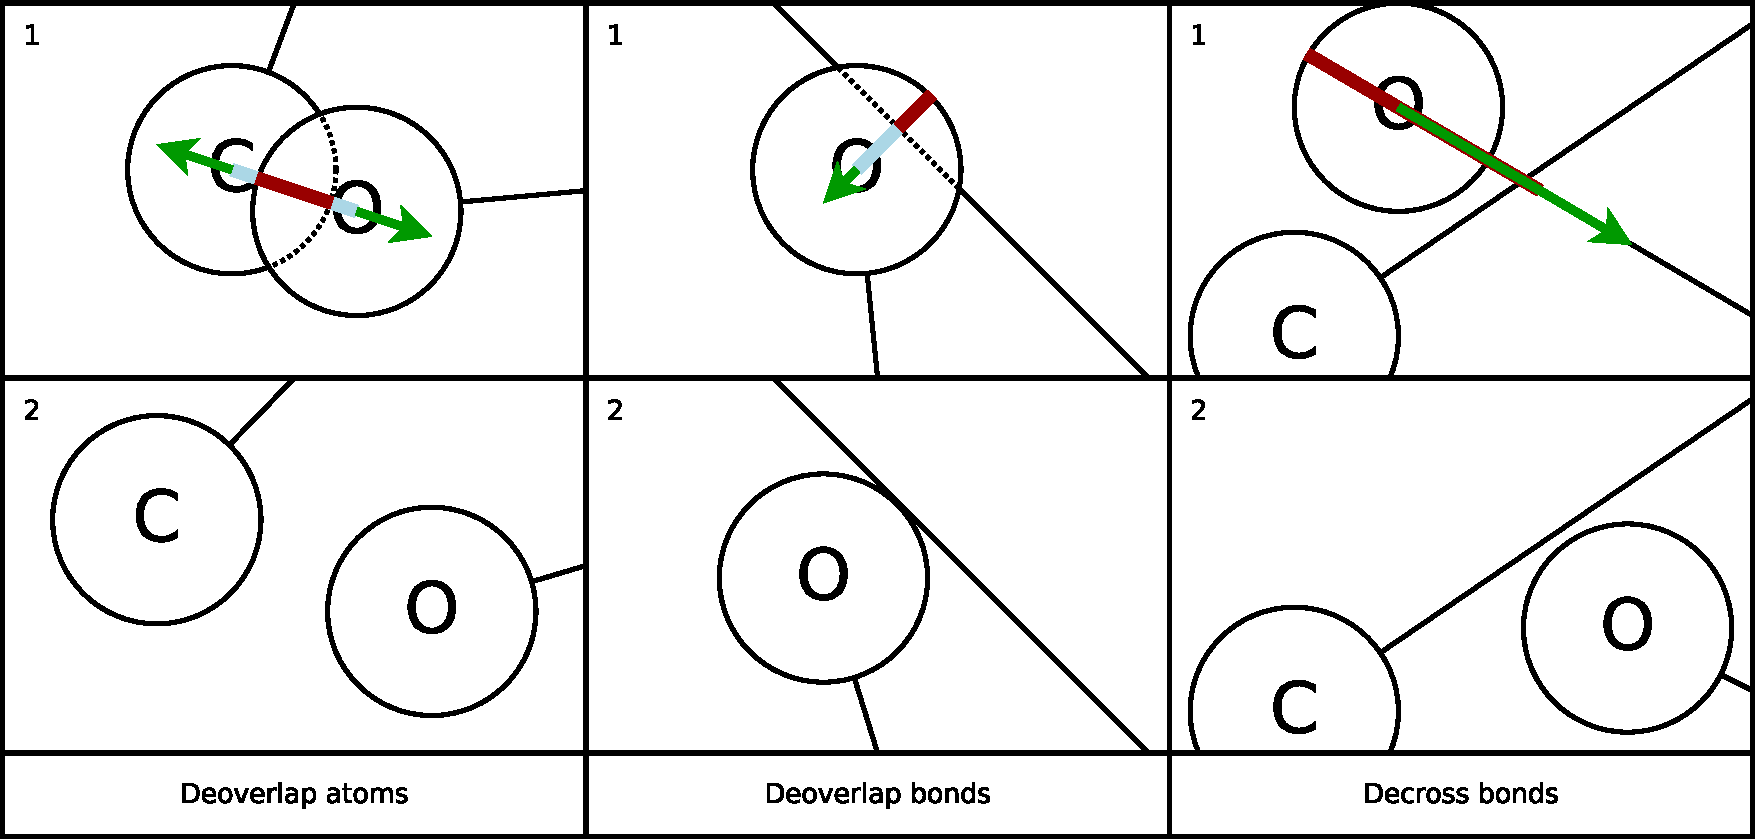
\includegraphics[width=\textwidth]{img/deoverlap.pdf}
\caption{Concepts of deoverlap.}
\figlab{impl_deoverlap}
\end{figure}

In order to solve atoms overlapping bonds, the perpendicular distance from the atom centre to the bond needs to be calculated. When this distance is smaller than the atom radius, the atom needs to be moved along the perpendicular for a distance that is equal to the overlap distance. This will put the atom right next to the bond.

The third and final type of deoverlapping, the so-called decrossing of bonds, is also the hardest one. First, it needs to be determined if the two bonds intersect each other. When that is the case, the intersection point needs to be found. The overlap distance here is equal to the distance from the atom centre to the intersection point, plus the radius of the atom. One of the atoms then needs to be moved along its bond for a distance that is equal to the overlap distance, in order to solve the crossing bonds.

Unfortunately, solving one occurrence of overlap could result in overlap occurring in a different place, as moving an atom could potentially move it on top of another. Therefore, the deoverlap process will need to repeat itself to solve all overlap in the molecule. However, it is possible that the solution of one overlap occurrence is the exact opposite of another, which means that, after two iterations, the situation will be exactly the same as it was initially. In order to prevent the deoverlap process from going into an endless loop because of this, a time limit~(set to half a second by default) has been built in, after which the deoverlapping will stop.


\subsection{Parameterisation}
In order to find the best interaction design for \oframp, two different interaction designs of it have been made. In order to allow for easy implementation of these different versions, a \verb|Behavior| interface\footnote{\texttt{JavaScript}, as of \texttt{ECMAScript} 5, does not have real interfaces, but the \texttt{Behavior} object acts as one.} has been created~(see \figref{oframp_class}). When a new behaviour for the system is designed, implementing this is as easy as making an implementation of that interface. As each interaction design also needs to have its own demo mode, the \verb|Demo| has been implemented as an interface as well. Implementing a demo mode for a different interaction design is therefore just as easy.


\subsection{Downloading results}
\seclab{impl_downloading}
When the user feels he is completely done, he can download the resulting parameterisation of the molecule by clicking the `Download' button at the top of the page. This will give him the result in the \verb|LEMON Graph File|~(LGF) format~\cite{dezso2011lemon}. This format has been chosen as it is used by, among others, the fragment finding system~(see \secref{impl2_omfraf}), and because it is a flexible format that can easily be generated. This file will contain all atoms' element types, \verb|IACM| number, and charge, as well as all bonds between the atoms.


\subsection{Modifying visualisation parameters}
In order to allow for modification of visualisation parameters at runtime, a slightly modified version of the \verb|JavaScript| library \verb|dat-gui|~\cite{data2011dat} has been used. This library can automatically generate a user interface from a \verb|JSON| object that contains the settings. Additionally, it can be provided with an object that contains various settings for the interface itself, such as which widget to use, and change event handlers.



\section[\oapoc]{The Online tool for Atom Position Calculations}
\seclab{impl2_oapoc}
Provided with a molecule data string~(MDS) and optionally a format specification for that string, \oapoc{} will provide detailed molecule data~(e.g. atoms, atom positions, bonds) represented by the MDS. Internally, \oapoc{} uses the \verb|Open Babel| program \verb|obabel| to convert the MDS to the \verb|Mol2| format. This format has been chosen as it can easily be parsed and contains information on atom positions and bonds. Furthermore, it does not leave out the $H$ atoms, which some other formats do. For some applications this is fine, but for \oframp{} it is required to have all $H$ atoms.

The data that \verb|obabel| returns will be parsed and converted to a \verb|JSON| object, such that it can be sent to the client running \oframp. Additionally, \verb|IACM| atom types are calculated, following the algorithm presented by Malde~et.~al.~\cite{malde2011automated}. These atom types are needed later to be able to find matching fragments for the molecule.


\subsection{From ATB}
When an \verb|ATB ID| is supplied to \oapoc, the accompanying molecule data string will be retrieved from the ATB. For all its molecules, the ATB stores a \verb|PDB| file, which is one of the formats that \oapoc{} supports. This file will be downloaded, and its contents will be used as the MDS for finding the molecule data.



\section[\omfraf]{The Online tool for Molecule Fragment Finding}
\seclab{impl2_omfraf}
\omfraf{} is the system that is responsible for retrieving matching fragments for the examined molecule. First, fragments will need to be generated, after which they can be queried. Additionally, it is possible to retrieve information about the available repositories. All of this will be discussed in the next sections.

\subsection{Getting the repositories}
In order to be able to select a repository, the user needs to know what repositories are available. As can be seen in \figref{network_diagram}, a list of repositories can be retrieved by sending an empty \verb|JSON| object to \omfraf's \verb|/repos| URL. As of now, this list consists of only the repository titles, but this may be extended later.

\subsection{Generating fragments}
\seclab{impl2_generating}
Before any fragments can be found, all matching fragments for the molecule need to be generated. In \omfraf, fragments are generated using El-Kebir's \verb|fragments| tool from the \verb|mop| project~\cite{elkebir2014molecule}. As can be seen in \figref{network_diagram}, this tool has been wrapped in a program called \verb|fragment_generator|. This requires the input of a \verb|JSON| object containing a molecule, and optionally a repository and shell size.

For every molecule in the provided repository, \verb|fragment_generator| will retrieve the matching fragments with the input molecule using \verb|mop/fragments| and transform them into a slightly more manageable format. It will then combine the fragments of all molecules and store them to disk in the so-called \omfraf{} Fragments File~(OFF) format. The name of this file will be sent back to the \oframp{} user, such that he can query for fragments later. Along with the fragment file's name, a list of atoms for which no matching fragments could be found is sent to the user, which will allow for indicating these atoms in the molecule visualisation~(see \secref{impl_completing}).


\subsection{Finding fragments}
\seclab{impl2_finding}
Once a molecule's fragments have been generated, the user of \oframp{} will be able to start the parameterisation process. The atom(s) he selects, combined with the OFF filename will be sent to \omfraf, which will invoke the \verb|fragment_finder|. This program will load the fragments from the OFF file, and select those in which \emph{all} selected atoms are present. Those fragments will be ordered based on the score that was assigned to them by the \verb|fragments| tool, and are returned to the \oframp{} front-end such that they can be used in the parameterisation process.
